% REMEMBER: You must not plagiarise anything in your report. Be extremely careful.

\documentclass{l4proj}

    
% put any additional packages here
\usepackage{amssymb, amsmath, amsthm}
\usepackage{subcaption, hhline, multirow}
\usepackage{enumitem}

%==============================================================================
%% Commands 
\theoremstyle{definition}
\newtheorem{definition}{Definition}[section]

\newtheorem{proposition}{Proposition}[section]
\newtheorem{example}{Example}[section]

\DeclareMathAlphabet{\mathcal}{OMS}{cmsy}{m}{n}

\newcommand{\codefont}[1]{{\fontfamily{lmtt}\selectfont #1}}

\setitemize{noitemsep}
%==============================================================================

\begin{document}

%==============================================================================
%% METADATA
\title{An Analysis on the Robustness of Watermarking Generative Text}
\author{Samuel Jackson}
\date{\today}

\maketitle

%==============================================================================
%% ABSTRACT
\begin{abstract}
    \textbf{Every abstract follows a similar pattern. Motivate; set aims; describe work; explain results.}
    \vskip 0.5em
    Given the rise of LLMs and the growing power of malicious content-generation, 
    methods of identifying and authenticating machine-generated content has become a necessity. 
    This paper aims to investigate the robustness of modern techniques in watermarking Transformer-based LLMs at inference through paraphrasing attacks. The paper presents evidence of poor defence in large documents against paraphrasing attacks
    where even a simple paraphraser can reduce detect-ability by ??\%.
\end{abstract}

%==============================================================================

% EDUCATION REUSE CONSENT FORM
% If you consent to your project being shown to future students for educational purposes
% then insert your name and the date below to  sign the education use form that appears in the front of the document. 
% You must explicitly give consent if you wish to do so.
% If you sign, your project may be included in the Hall of Fame if it scores particularly highly.
%
% Please note that you are under no obligation to sign 
% this declaration, but doing so would help future students.
%
\def\consentname {Samuel Jackson} % your full name
\def\consentdate {\today} % the date you agree

\educationalconsent


%==============================================================================
\tableofcontents

%==============================================================================
%% Notes on formatting
%==============================================================================
% The first page, abstract and table of contents are numbered using Roman numerals and are not
% included in the page count. 
%
% From now on pages are numbered
% using Arabic numerals. Therefore, immediately after the first call to \chapter we need the call
% \pagenumbering{arabic} and this should be called once only in the document. 
%
% Do not alter the bibliography style.
%
% The first Chapter should then be on page 1. You are allowed 40 pages for a 40 credit project and 30 pages for a 
% 20 credit report. This includes everything numbered in Arabic numerals (excluding front matter) up
% to but excluding the appendices and bibliography.
%
% You must not alter text size (it is currently 10pt) or alter margins or spacing.
%
%
%==================================================================================================================================
%
% IMPORTANT
% The chapter headings here are **suggestions**. You don't have to follow this model if
% it doesn't fit your project. Every project should have an introduction and conclusion,
% however. 
%
%==================================================================================================================================
\chapter{Introduction}
    \label{chap:introduction}
    
    \pagenumbering{arabic} 

    \section{Motivation}
        Generative AI has already been used to influence political opinions and continues to create scepticism and fear amongst the general public \citep{leffer2024anxiety}. Existing Large Language Models (LLMs), such as ChatGPT, can provide help with homework, display human-like emotion and unknowingly misinform users.
    
        The capacity for misinformation with the new-found capabilities of LLMs is significant enough to spur governmental action \citep{whitehouse2023ai} and cause leaders of tech world to seek a petition slowing the progress of AI development \citep{life2024pauseai}.
        
        In an effort to combat the intentional and unintentional dissemination of misinformation, techniques for identifying the use of LLMs has become a focus for many people \citep{kirchenbauer2023watermark, mitchell2023detectgpt, grinbaum2022ethical}. The growing difficulty in detection methods \citep{sadasivan2023aigenerated} has led to research into placing unique signatures into content created by large language models \citep{openAIclassifier}.

    \section{Watermarking}
        Techniques for embedding signatures, known as watermarking, have been growing rapidly in the last year. One particular technique, known as the Maryland Watermark, proposed biasing the generation towards certain words \citep{kirchenbauer2023watermark}. Some techniques have further developed the Maryland Watermark ideas \citep{liu2024semantic}, whereas some place rare Unicode characters within the generated text \citep{sato2023embarrassingly} or store outputs from the language models and view watermarking as a retrieval problem \citep{krishna2023paraphrasing}.
        
    \section{Problem}
        However, the existence of these watermarks has not been sufficient in ensuring that we can identify the machine-generated content. In fact, methods of removing these watermarks are prevalent and certainly exist. 

        We will be discussing the quality of the watermark and how easy it is to remove the ownership-identifying features of watermarked text. To respect the depth of this paper, we focus our analysis around the Maryland Watermark. We summarise our problem into a single question: ``To what extent is the Maryland Watermark technique robust against bad actors?''

        The investigation into our question will be completed through attempting to remove the watermarked from documents through various techniques. Chapter 2 will be providing the necessary background into watermarking and watermark removal techniques. Chapter 3 will follow immediately with the implementation of our research method, focused on differing types of paraphrasing. Chapter 4 will present our results and attempt to answer our question stated above. Finally, our paper is completed with a conclusion, summarising the paper and highlighting our key results.

%==================================================================================================================================
    
\chapter{Background}
% Fix here.
Transformers have realised the creation of incredibly powerful large language models, such as ChatGPT. The potential of these models has led to governmental action on ensuring the safety of AI \citep{whitehouse2023ai}. One such safety method is watermarking text as it can allow us to correctly prescribe the author of a document to a large language model, if necessary. This chapter will provide an overview of how LLMs generate text alongside an insight into recent literature on text-watermarking as well as methods of removing such watermarks. 

The sections are split to respect the order of text generation, watermark generation and watermark removal, to aid the reader. The watermark generation and removal steps contain literature surveys of relevant techniques. 

In particular, the literature survey acts as inspiration in our approach to the understanding the problem. Whilst not all techniques that are discussed are used in this paper, they are certainly relevant in terms of understanding our problem.

\section{Text Generation}
    As our discussion is focused on watermarking generated text, we first provide an explanation into how text is produced from Transformer-based LLMs.

    This section will go over the concepts behind providing text to models, as well as how the model chooses the next word in a sentence.
    
    \subsection{Tokenisation}
        \label{sec:tokenisation}
        In order to process and train language models, we must provide a structure to our textual data. In this section we discuss how text is prepared for large language models through a process known as tokenisation.
        
        An element of a textual dataset is known as a \emph{document}. Through tokenisation, we structure our document into a list of \emph{tokens}.

        \begin{definition}[Token]
            A \emph{token} is a sequence of characters, often referring to a word or a subword.
        \end{definition}

        The choice of tokens over words is due to the dramatic scale of unique words. Tokens allow for a reduction of dimensions and becomes more manageable for computation. Although rule-based tokenisation exists, language models currently use trained tokenisation models. Tokenisation models are developed through methods like training a Byte Pair Encoding (BPE) tokeniser \citep{Gage1994ANA, sennrich2016neural} on a text corpus. As seen in Figure~\ref{fig:tokenisation-process}, a tokenisation function takes a string as input and produces a list of tokens, based on the vocabulary. 
        
        \begin{figure}[ht]
            \captionsetup[subfigure]{labelformat=empty}
            \centering
            \begin{subfigure}{\textwidth}
                \includegraphics[width=\linewidth]{images/background/tokenisation-process-mistral.png}
                \caption{\emph{(a)}}
                \label{fig:tokenisation-process-mistral}
            \end{subfigure}

            \begin{subfigure}{\textwidth}
                \includegraphics[width=\linewidth]{images/background/tokenisation-process-bert.png}
                \caption{\emph{(b)}}
                \label{fig:tokenisation-process-bert}
            \end{subfigure}

            \caption{Figure visualises the potential differences in tokenisation functions. Figure (a) was completed using the \codefont{Mistral-7B-v0.1} tokeniser \citep{jiang2023mistral}, a BPE tokeniser. Figure (b) was completed using the \codefont{bert-base-uncased} tokeniser \citep{DBLP:journals/corr/abs-1810-04805}, a WordPiece tokeniser.}
            \label{fig:tokenisation-process}
        \end{figure}

        \begin{definition}[Vocabulary]
            A \emph{vocabulary} is the collection of tokens recognised by a tokenisation function.
        \end{definition}

        Importantly for our discussion on watermarking language models, the training of these tokenisation models generates a \emph{unique} vocabulary dependent on the text corpus. The difference in recognised tokens is evident when comparing the lists of tokens in Figure~\ref{fig:tokenisation-process}. The tokenisation uniqueness is propagated through the transformer-based architecture.

        
    
    \subsection{Generation Strategies}
        \label{sec:decoder-generation}
        Text generation is treated as a predict-next-token task. We choose to only look at the previous tokens and consider which token is most likely to next appear. This task is known as Causal Generation. In attempt to respect the depth of this paper, I will not dive deep into the model architecture but this section will discuss model outputs and generation techniques.

        Causal Language Models, models used for Causal Generation, produces a probability distribution from which we choose the next token. The probability distribution is obtained from applying the Softmax function to a collection of values, which we call \emph{logits}. 

        The created probability distribution is used for multiple generative strategies which include greedy-generation, multinomial sampling, and top-$p$ sampling.

        Each generation strategy serves a different purpose. Greedy-generation is a fast deterministic technique which simply chooses the token with the highest probability in the distribution. The deterministic nature means that the model will always produce the same output. On the other hand, top-$p$ sampling is a method which randomly chooses a token from the set of the highest tokens such that the sum of the token probabilities is less than or equal to $p$. Top-$p$ is helpful in providing more diverse text, whilst also allowing the parameters to avoid potentially strange tokens.

\section{Generating Watermarks}
    \begin{definition}[Watermark]
        A \emph{watermark} is a faint figure or signature designed to represent ownership or authorship.
    \end{definition}

    Watermarks are widely present within society with examples ranging from an American dollar bill to a music producer having an audio tag. In this section, we look towards recent literature which covers subtle methods of watermarking while attempting to adhere to the primary goals of watermarking.

    \begin{figure}[ht]
        \centering
        \includegraphics[height=3.5cm, width=1\linewidth, keepaspectratio]{images/background/dbill-highlighted.png}
        \caption{Figure shows an \$100 dollar bill, with a red circle highlighted a watermarked portion. The detection of the highlighted watermark requires holding the bill up to light and revealing a (second) face of Benjamin Franklin \citep{bep2013dollar}.}
         \label{fig:dbill-watermark} 
    \end{figure}
         
    Given the purpose of watermarking generative content, there are the following primary goals that an AI text watermark aims to achieve:
    \begin{itemize}
        \setlength\itemsep{0.5em}
        \item \textbf{Robust} - Capable of withstanding attempts to remove watermark.
        \item \textbf{Agnostic} - Information beyond generated text is not required for detection.
        \item \textbf{Imperceptible} - The watermark should not be visible, be it a change in quality or a written signature.
    \end{itemize}

    These requirements are designed to encourage universal watermarking techniques due to the constant growing number of large language models and changing architecture decisions.
    
    \subsection{Maryland Watermark}
        \label{sec:maryland-watermark}
        \citet{kirchenbauer2023watermark} proposes a new method of watermarking text which takes advantage of the probabilistic nature of text generation. This section will go over the ideas of the Maryland Watermark, a technique which laid the foundations of watermarks in LLMs at the time of this paper.

        Due to the nature of casual generation, each token is generated procedurally from the vocabulary. The Maryland paper proposes splitting the available vocabulary for each token. The split lists are labelled a \emph{green} list and a \emph{red} list, where green tokens are used for detection. Notably, the splitting is a random sort and partition based on the hash of the last token.

        In particular, there are two primary watermarking techniques, \emph{Hard Watermarking} and \emph{Soft Watermarking}. Hard Watermarking only allows the causal model to select tokens from the green list whereas Soft Watermarking simply increases the probability of the green tokens within the probability distribution. Figure~\ref{fig:soft-watermarking-process} outlines the technique and the change that the Soft Watermarking process has on the probability distribution.

        \begin{figure}
            \centering
            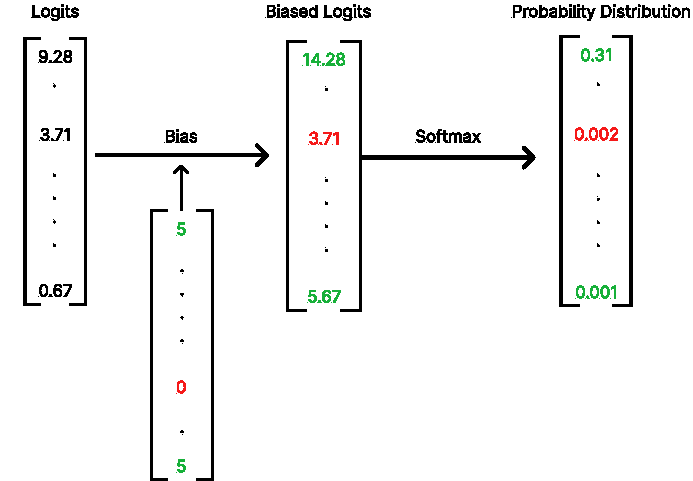
\includegraphics[width=0.5\linewidth, keepaspectratio]{images/background/biasing-process.pdf}
            \caption{Figure portrays the Soft Watermarking process where the bias value is 5. Visualisation of adding the bias to green tokens and altering the final distribution for all the tokens.}
            \label{fig:soft-watermarking-process}
        \end{figure}

        As opposed to Hard Watermarking, Soft Watermarking provides parameters that determine the strength of the watermark. The parameters are $\delta$, the logit bias, and $\gamma$ is the fraction of the vocabulary which is the green list. Typical values for $\delta$ and $\gamma$ are within the ranges $[1, 10]$ and $[0.25, 0.5]$, respectively.

        \citet{kirchenbauer2023watermark} provides an analysis on the Soft Watermarking technique, outlining the performance on differing bias and generation strategies. Without describing the necessary metrics, the paper shows that watermarking, with no detection-errors, can be achieved at reasonable strengths of watermarking whilst maintaining quality of the text.
        
    \subsection{Easymark}
        \label{sec:easymark}
        As opposed to complicated and robust watermarking techniques, like described above, \citet{sato2023embarrassingly} beautifully proposes simple watermarks that are not intended to survive bad actors. This portion will briefly go over the watermarks as well as highlight the argument of watermark futility from \citet{sato2023embarrassingly}.

        The provided watermarks are labelled as \emph{Whitemark}, \emph{Variantmark} and \emph{Printmark}. All of the methods are weak to bad actors using attacking techniques such as word-replacement, paraphrasing and homoglyph removal however the method of watermarking leads to no degradation in perplexity. The entire family of watermarks proposed are variations on manipulations of Unicode characters, whether it be replacing whitespace characters or replacing characters with rarer Unicode siblings.

        \begin{figure}[ht]
            \centering
            \includegraphics[width=1\linewidth, height=2.7cm, keepaspectratio]{images/background/inf-ligature.png}
            \caption{Figure showcasing one of watermarking methods, Printmark. The characters `f' and `i' have been changed to the Unicode ligature U+FB01, providing a signature as the ligature is uncommon.}
            \label{fig:fi-ligature}
            \nocite{infinity-ligatures-pict}
        \end{figure}

        Within the paper, \citet{sato2023embarrassingly} discusses the strength of bad actors and describes a statistical analysis as to why a perfect watermark is impossible. In fact, the paper proposes that it is more prudent to place a low-effort watermark and not place too much confidence within watermarks. 

        Paired with our research questions, our discussion on current watermarking robustness will hopefully bring light to the worthiness of watermarking. 

        We will not be discussing Easymark further within this paper but it is worthy reading the paper by \citet{sato2023embarrassingly}.
    \subsection{Retrieval defence}
        \citet{krishna2023paraphrasing} proposes a retrieval-based defensive technique, designed to hold strong against paraphrasing attacks. This section will cover the principle ideas and primary results surrounding defence that are discussed in the paper. 

        Contrary to the other watermarking methods, this is a defensive technique that requires no generative-stage changes to the LLMs. The primary idea is to store AI-generated documents into a database and determine if a document is AI-generated by completing a retrieval call into the database.

        % Results at this stage are unknown to reader
        This method achieves significant results with the evaluation taking place over multiple models. Before paraphrasing, retrieval detection has an accuracy of 100\% on 1\% FPR and after strong machine-paraphrasing, there is more than 96\% accuracy across all models. This is compared to the Maryland watermark which achieves 55.8\% accuracy, a starkly lower performance.
        
        Notably, for these results, however, is that the retrieval corpus matches exactly the initial generated documents and the retrieval technique is dependent on a reliable database. Furthermore, differing language models may require different databases which could make the retrieval query an expensive cost. 
        
    \subsection{Other Watermarking Techniques}
        \label{sec:other-watermarks}
        Although I will not have the time to experiment with these techniques, the following papers present relevant and interesting watermarking methods. This section will only provide a high-level overview but I strongly recommend reading these papers.

        As opposed to altering the sampling distribution, \citet{kuditipudi2023robust} suggests a watermarking method that provides a sequence of random numbers, known as the \emph{watermarking sequence}. For each token, we choose the next token through an element of the watermarking key sequence, as opposed to sampling or other generation strategies. The randomness of the watermarking sequence is intended to emulate the sampling process, maintaining the imperceptibility property. 

        \citet{liu2024semantic} proposes a dynamic bias which considers the semantic meaning of the previously generated tokens, as opposed to a fixed bias like the \hyperref[sec:maryland-watermark]{Maryland Watermark}. The technique consists of an embedding model, a custom watermark model as well as a language model. The custom watermark model, $T$, receives embeddings as input and produces logits, $P_T$. Paired with the logits produced by the language model, $P_M$, we create a new distribution $P_{\hat{M}} = P_M + \delta P_T$, where $\delta$ weights the distribution $P_T$. A visualisation of this process is provided in Figure~\ref{fig:embedding-watermark-process}

        \begin{figure}[ht]
            \centering
            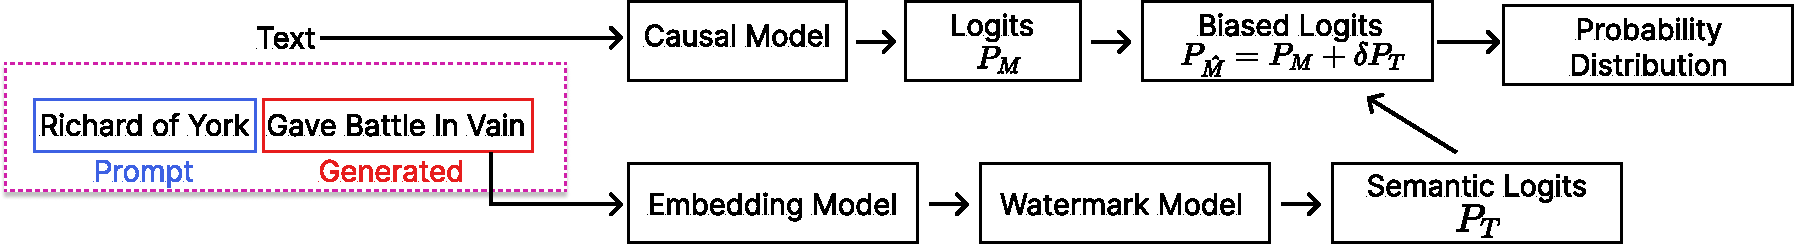
\includegraphics[height=5cm, width=\linewidth, keepaspectratio]{images/background/embedding-watermark-process.pdf}
            \caption{Figure highlights the watermarking process proposed by \citet{liu2024semantic}. The embedding model only takes tokens from the already generated tokens as input, highlighted in red, whereas the causal model uses all the text, prompt and generated, to produce its logits. Both sets of logits are linearly combined, with a weighting $\delta$, to create a biased probability distribution.}            \label{fig:embedding-watermark-process}
        \end{figure}
        
\section{Attacking Watermarks}
        No matter the robustness of a watermark, methods of removing the watermark are real threats. We call attempts to remove a watermark, no matter the removal method, an \emph{attack} on the watermark.

        Within this stage, we will discuss the word-replacement strategy, paraphrasing and translation-attacks. Specifically, we highlight a number of techniques that we will be applying for our method of investigation alongside relevant literature which prove other successful methods of attacking.

    \subsection{Word Replacement}
        A classic and simple technique is \emph{word-replacement}. In this section, I will cover the motivation behind word-replacement as well as an overview of the technique.

        This is perhaps the most primitive form of attacking. As opposed to restructuring a sentence or paragraph, we replace words with suitably appropriate words. We are motivated to complete word-replacement because it is a low-cost approach, comparatively, given the lack of an intensive large language model. Furthermore, the word-replacement algorithm has the potential to remove the so-called `green tokens', reducing the chance of being detected as watermarked.  

        This method is dependent on a Part of Speech (POS) tagger model. A POS model is trained to give grammatical structure to words. This helps us understand how to replace a particular word. Figure~\ref{fig:word-replacement-process} provides a clear outline of the method, containing the Part of Speech tagging. 

        \begin{figure}[ht]
            \centering
            \includegraphics[height=5cm, width=1\linewidth, keepaspectratio]{images/background/word-replacement-process.pdf}
            \caption{Figure displays the word replacement process where 20\% of all words are replaced with similar words, with respect to their part of speech. This process is completed by my word replacement method and the Flair Part of Speech Tagger \citep{akbik2018coling}.}
            \label{fig:word-replacement-process}
        \end{figure}
        
        The major flaw in this method is the lack of semantic understanding. The benefit that transformers provide all large language models is thrown away through the use of this technique and drastically reduces the quality of the text.
        
        Variations of this technique exist, such as only replacing adjectives with respect to the POS tagger. These variations are designed to compensate for the lack of semantic understanding that a word-replacement algorithm has.

        Whilst the method comes with many flaws, this paper will discuss an analysis of this attack, something which is novel amongst current research papers.
    
    \subsection{Paraphrasing}
        Given that the techniques of watermarking are focused around the particular words used within a generated document, we aim to remove those `bad' words, whilst maintaining or improving the clarity of the original meaning. However, without knowing the watermarked words, word-replacement might not be sufficient. 

        In this section, we discuss paraphrasing as an approach that could remove the green tokens whilst maintaining the quality of the original text. We extend this discussion into large language models, as well as recent papers surrounding paraphrasing attacks.

        \begin{definition}[Paraphrase]
            \label{def:paraphrase}
            To repeat something written or spoken using different words, often in a humorous form or in a simpler and shorter form that makes the original meaning clearer (Cambridge Dictionary, 2024). % Perhaps I should cite this in references
        \end{definition}

        As can be seen in Example~\ref{example:paraphrase}, we often restructure sentences for clarity which is something that word-replacement is incapable of doing without a degree of semantic understanding.

        \begin{example}
            \label{example:paraphrase}
            The two sentences below are examples of paraphrases.
            \begin{enumerate}[label=(\alph*)]
                \item I take my dog on a walk in Central Park each Wednesday. 
                \item Every Wednesday, I walk my dog in Central Park.
            \end{enumerate}
            These two sentences maintain semantic meaning while holding a different sentence structure. 
        \end{example}

        In recent literature, \citet{krishna2023paraphrasing} discusses the attacks of paraphrasing by providing a paraphrase language model known as DIPPER. Through finetuning, this model is a paragraph-context paraphrase model with variable parameters. These parameters determine the degree of order and lexical change performed by the paraphrasing. A change in order refers alterations to the grammatical structure of a document whereas a lexical change denotes replacing particular words, choosing a synonym for an adjective.

        Within the DIPPER paper, results of the paper convey the decreasing detection accuracy as the order and lexical parameters increase. The paper's highlighted statistic shows that where false detection of human-text as AI-text is at 1\%, the DIPPER paraphraser drops accuracy of DetectGPT from 70.3\% to 4.6\%.

        Similarly, in other literature, \citet{sadasivan2023aigenerated} investigates recursive paraphrasing on watermarked documents with two models, DIPPER and a LLaMa-based chat model. In particular, the analysis takes place on generated documents of approximately 300 tokens. 

        The paper reports results of clear degradation in detection through the iterations of DIPPER-based paraphrasing. With the case where false-detection of human-text as AI-text is at 1\%, the chance that a watermarked document is detected drops from 99.8\% in the original document to 30.9\% in the third paraphrase. This is significant change at minimal cost, as reported by \citet{sadasivan2023aigenerated}, where the cost is discussed with respect to the perplexity metric. 

    \subsection{Translation-Based Paraphrasing}
        \citet{he2024watermarks} provides a deep investigation into the process of using translation to remove watermarks. As opposed to training a new paraphraser, \citet{he2024watermarks} utilises existing translation models in order to paraphrase. This section will give a brief overview as to how this works and the performance of the technique. 

        % Maybe not say principal idea so much, perhaps switch it up
        As can be seen in Figure~\ref{fig:translation-removal-process}, the principal idea behind translation-based paraphrasing is twice-translation, going to another language and back. 

        \begin{figure}[ht]
            \centering
            \includegraphics[height=3.5cm, width=1\linewidth, keepaspectratio]{images/background/translation-removal-process.pdf}
            \caption{Figure above displays the translation attacking process with twice translation involving English and Spanish. Translations were completed with the \texttt{opus-mt-en-es} and \texttt{opus-mt-es-en} models respectively \citep{TiedemannThottingal:EAMT2020}.}
            \label{fig:translation-removal-process}
        \end{figure}
        
        This method is particularly effective because the architecture behind paraphrasing and translation is the same: Sequence-to-Sequence (Seq2Seq). The Seq2Seq architecture is a decoder which has access to all the tokens in a document, not just the previous ones. This drastically improves the performance of LLMs on tasks like summarisation as it takes different context into account. 

        \citet{he2024watermarks} outlines clear results which portray the efficacy of this technique. A highlighted result is, in the case of false-detection of human-text as AI-text is at 10\%, the chance that a watermarked document is detected drops from 99.2\% to 21.3\% after paraphrasing with this method. This is a noticeable change and shows that the translation attacks bring the performance of a random classifier. 

    \subsection{Other Attacking Techniques}
        Despite the number of these techniques, there does exist others that I will not be able to provide a deep background into within this paper.

        A technique which was previously mentioned was \emph{homoglyph removal}. This technique is used to counter embedding watermarks through ASCII and Unicode characters, a perfect counter to the watermarking concepts in Section~\ref{sec:easymark}. The technique consists of a script which tests each character against Unicode pairs, replacing uncommon variations of a character to the norm. 

        \emph{Spoofing} documents is an interesting technique of \emph{attacking the validity} of a watermark. \citet{sadasivan2023aigenerated} shows that some watermarking methods are vulnerable to purposely making human-documents seem watermarked. This approach does not aid in removing watermarks from machine-generated documents but it reduces the credibility of a watermark. Without trust in the watermark, it is hard to justify its use in authorship.

        Both of these techniques are particularly effective techniques but they will not be further discussed in this paper as they are only applicable to certain watermarks. 

\section{Approach}  
    Following all of this background, we summarise the primary points that will be used for the rest of our paper. Within the rest of this paper, we shall be generating documents and attacking them through three primary methods.

    Our attacking methods consist of:
    \begin{itemize}
        \setlength\itemsep{0.5em}
        \item \textbf{Paragraph-Based Paraphrasing}: Paraphrasing the entire document, supplying the entire context. 
        \item \textbf{Sentence-Based Paraphrasing}: Paraphrasing each sentence within a document, only supplying context of the given sentence.
        \item \textbf{Word Replacement}: Changing words within the document to similar words.
    \end{itemize}

    \subsection{Problem Phrased}
        Our problem can be succinctly defined in the following question: ``To what extent is the Maryland Watermark technique robust against bad actors?''

        This paper breaks down that question into 4 smaller sub-questions. These sub-questions form our research questions for the paper and what we aim to understand.
        \begin{enumerate}[label={\textbf{RQ\arabic*}:}, leftmargin=4em]
            \label{sec:research-questions}
            \item Does paraphrasing recursively degrade accuracy in detection of the Maryland Watermark?
            \item Is sentence-based paraphrasing more effective than paragraph-based paraphrasing when dealing with removal of the Maryland Watermark?
            \item Is a low-cost, word-replacement algorithm sufficient to remove the Maryland Watermark? 
            \item Are the attacking methods feasible for use within an academic context with respect to the Maryland Watermark?
        \end{enumerate}

%====================================================================================================
    
\chapter{Methods}
\label{chap:method}

With the aim of understanding the robustness of watermarks in generative text, we discuss our method that takes us from the generation of watermarked documents to the evaluation of attacked documents.

\section{Overarching Approach}
    Before detailing all the design choices, I present the overarching implementation of our research method to aid in following along amongst the choices. The visual in Figure~\ref{fig:method-flow-chart} is provided to further assist in understanding the approach.

    \begin{figure}[ht]
        \centering
         \includegraphics[height=10cm, width=1\linewidth, keepaspectratio]{images/methods/research-process.pdf}
        \caption{Figure displaying the research processing, highlighted into their respective stages.}
        \label{fig:method-flow-chart} 
    \end{figure}
    
    The approach begins with creating watermarked documents through a large language model, given a dataset of prompts. These watermarked documents will be paired alongside non-watermarked documents, written by the same model, without the watermark. The non-watermarked documents serve as a benchmark, so as to better understand the impact of the watermark.

    Consequently, these essays are passed through our chosen attacking methods. These attacking methods will be two variants of paraphrasing as well as word-replacement. 

    Finally, we will evaluate the watermark quality of all the documents, which will include all the attacked documents as well as the original documents. There will be two primary evaluation stages with further evaluation metrics to help display the results in a meaningful representation.

\section{Generation Stage}
    \subsection{Dataset}    
        To generate our watermarked documents, prompts had to be provided to a causal language model. To match our causal model, the prompts were selected to be in the form of instructions or tasks. These prompt also came alongside human-written student essays. The student essays are useful in providing benchmarks for some evaluation metrics, such as perplexity.
    
        Kaggle, a data science platform, hosted a competition focused on detecting AI generated text \citep{llm-detect-ai-generated-text}. As the competition was an AI focused task, people created additional datasets to aid in finetuning. One such augmenting dataset is known as the DAIGT dataset, produced by \citet{Paullier2023-rx}, and is the dataset that will be used.

        The associated student essays were scraped from a separate Kaggle competition \citep{feedback-prize-english-language-learning}, guaranteeing that the essays are not AI-generated.

        The dataset is composed of three relevant columns: \emph{id}, \emph{text}, \emph{instructions}, with 2421 rows. The \emph{instructions} column refers to tasks given to students, where the paired \emph{text} column refers to the essay produced by a student according to the task.

        \begin{table}[ht]
            \centering
            \small 
            \begin{tabular}{@{}l|p{0.38\linewidth}|p{0.38\linewidth}@{}}
                \toprule
                id & text & instructions \\ \midrule
                6060D28C05B6 & Some schools in United States ofter classes from home because is good option to students . Some scho... & Task: Write a persuasive essay on whether or not classes from home should be offered as an option f... \\ \cmidrule(r){1-3}
                60623DB5DE7A & Four-day work week, a remarkable idea to conserve energy and resources, some businesses have adopted... & Task: Research the advantages and disadvantages of a four-day school week and write an essay to det... \\ \bottomrule
            \end{tabular}
            \captionsetup{width=.95\textwidth}
            \caption{The above table displays 2 of the existing 2421 rows within the DAIGT dataset, where columns are cut for brevity and readability.}
            \label{table:dataset-sample} 
        \end{table}

        Current literature is focused on auto-generative prompting whereas I have decided to focus on instruct-style prompting. Instruct-style prompting, to the best of my knowledge, is not deeply investigated within this area hence it could lead to differing results. Although interesting, attempting to investigate both auto-generative and instruct-style prompting is outwith the scope of this project.
        
        Initial investigations were completed with the auto-generative style, using a dataset of one million articles \citep{Signal1M2016}, if you are inclined to re-evaluate results with a different prompting style.
        
    \subsection{Model}
        Current literature studying watermarks is typically using auto-generative and chat models \citep{pang2024attacking, liu2024adaptive, kirchenbauer2023watermark, sadasivan2023aigenerated}. This paper will use Mistral-7B-Instruct-v0.2 (Jiang et al. 2023), which is a 7 billion parameter model which has performed very well in a variety of benchmarks. It is an Instruct model, a model which is finetuned towards dealing with instruct-style prompts.

        From Figure~\ref{fig:prompting-method}, the prompting method is designed to reflect the instruct-nature required for the model. Instruct response, with an actual essay prompt from our chosen dataset.
        
        \begin{figure}[ht]
            \centering
            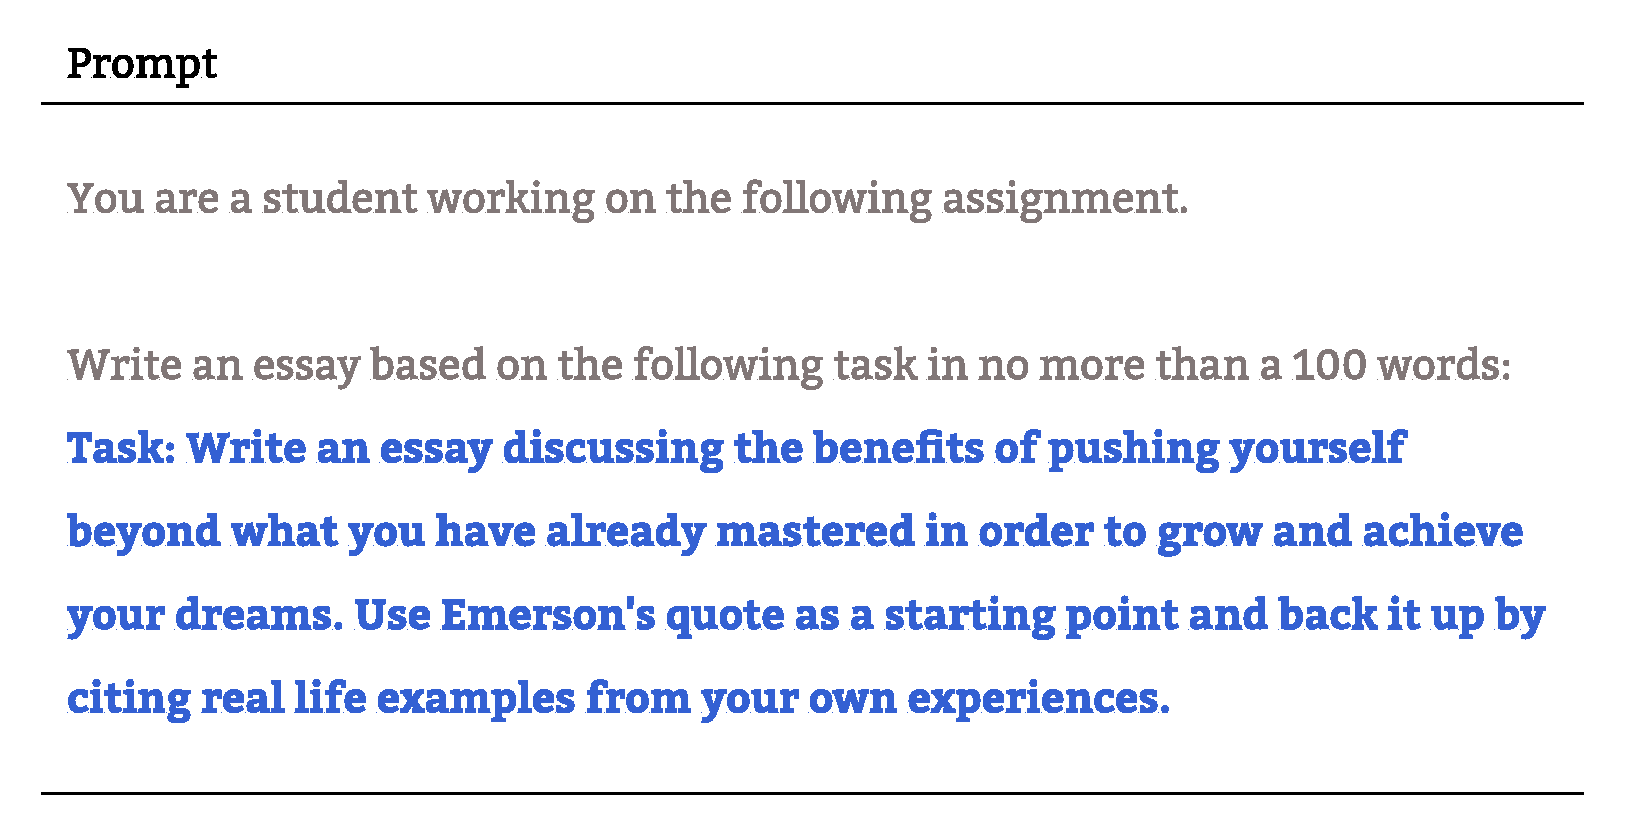
\includegraphics[height=6cm, width=1\linewidth, keepaspectratio]{images/methods/prompt-template.pdf}
            \caption{Figure portraying the prompting method used for the generation of watermarked essays, where the content in blue is a sample from the \emph{instructions} column in the DAIGT dataset. The grey text represents additional prompt text used to guide the model.}
            \label{fig:prompting-method}
        \end{figure}

        The chosen generation strategy was multinomial sampling, with the max number of new tokens generated set at 7500, to allow for potentially large documents. No other sampling strategies, such as top-$p$ were used, as we aimed to create the most diverse documents possible. 
        
    \subsection{Watermark}    
        \label{sec:watermark-implementation}
        We will be using the Soft Watermarking method, outlined in Section~\ref{sec:maryland-watermark}, as it is the watermark on which we have focused our research questions. 

        The Maryland Watermark was the ideal watermark as it is the original paper on the logit-manipulation-based watermarking. Other watermarking techniques are present, such as Easymark from Section~\ref{sec:easymark} or a Semantics-based watermark \citep{hou2024ksemstamp}, however these watermarks are not implemented to respect the breadth of this paper. 

        Our implementation is completed using the HuggingFace Python library \citep{wolf-etal-2020-transformers}, alongside code provided by \citet{kirchenbauer2023watermark}. This library provides an interface to the language model as well as the ability to manipulate logits at the generation stage, prior to the creation of the probability distribution, as outlined in Figure~\ref{fig:soft-watermarking-process}. 

        Specifically, we choose our bias and green list fraction to be $\delta = 5$ and $\gamma = 0.25$ respectively. This means that for the generation of each token, a quarter of the vocabulary are `green' tokens. Similarly, those `green' tokens will have a bias of 5 added to them. These parameters are in line with results from \citet{kirchenbauer2023watermark} and reflect a strong watermark that maintains a reasonable degree imperceptibility.

\section{Attacking Stage}
    In this section, I will be going over our attacking technique. In order to understand the robustness of watermarks, it is necessary to attempt watermark removal with a diverse range of methods. 

    As highlighted in Figure~\ref{fig:method-flow-chart}, we choose to paraphrase attack with a sentence-based and paraphrase-based paraphraser. Furthermore, we apply our word-replacement algorithm as an attacking method. All of the prior methods will be discussed in this section, in the listed order.

    The mentioned techniques precisely cover our research questions, \textbf{RQ1}, \textbf{RQ2}, \textbf{RQ3} and \textbf{RQ4}, which helps us answer our overarching questions of watermark robustness.

    \subsection{Paragraph-Based Paraphrasing}
        \label{sec:paragraph-paraphraser}
        Our attacking approach of paraphrasing with respect to the paragraph is based on the idea of supplying the maximal amount of context. With more context, the model is afforded greater potential to gleam the semantic meaning of a document. 
    
        To create a paragraph-based paraphraser, we choose a model with the same architecture as a translation model. \citet{krishna2023paraphrasing} proposes precisely this model, known as DIPPER. In fact, the paper discusses finetuning from dataset generation to a finetuned model. Unfortunately, due to computational constraints, we could not use the given model. As a result, we choose to create our own model, with the principles from this initial paper. For brevity, I will refer to this model as \emph{$p$-paraphraser}.
        
        We choose to finetune a Sequence-to-Sequence (Seq2Seq) model with a dataset of paragraph pairs. Google's T5 models are designed for transfer learning \citep{raffel2023exploring}, hence we look towards a variation of T5. The decided model ended up as a checkpoint model, \codefont{t5-efficient-large-nl32}. The suffix of this model refers to the number of transformer blocks, where 32 is larger than the norm. The large number of transformer block adheres to a Deep-Narrow architecture, a recommendation from \citet{tay2022scale}, the paper which produced these variation models.

        \citet{krishna2023paraphrasing} leverages the Par3 dataset \citet{Par3_2022} to create the dataset that I will be using, which I will refer to as kPar3. Par3 is a collection of books, translated by multiple authors. The paragraphs from each translation are collected and aligned, appearing as paraphrases. Figure~\ref{fig:par3-collection-process} provides a visual description of how the Par3 data is collected.

        

        \begin{figure}[ht]
            \centering
            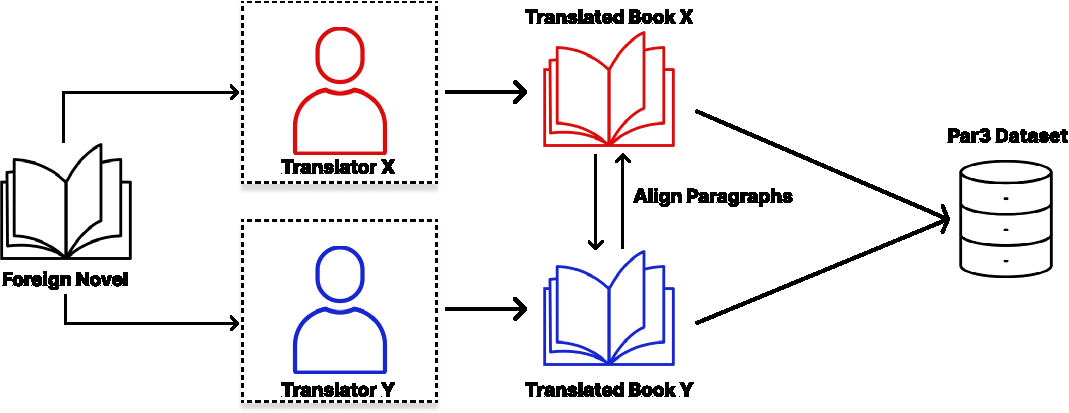
\includegraphics[width=1\linewidth, height=5cm, keepaspectratio]{images/methods/par3-collection-explanation.pdf}
            \caption{Figure describing how the Par3 data is created and produced. Figure is outlining that a famous book is translated by multiple distinct people. The respective translation paragraphs are aligned with each other and considered paraphrases.}
            \label{fig:par3-collection-process}
        \end{figure}

        The kPar3 dataset created documents that contained $\sim$6,000,000 paraphrase pairs, split between Google translated and the human translated described above. Within each section, there is further nondescript subsections. These subsections are composed of documents which provide context to the paraphrase and those that do not. The structure of the dataset is described in Figure~\ref{fig:kpar3-structure}. Each document starts with the arguments \emph{lexical} (L) and \emph{order} (O), as seen in Figure~\ref{fig:kpar3-sample-comparison}, where each argument only has values from the set \{0, 20, 40, 60, 80, 100\}. These arguments are included to impose an understanding of paraphrasing strength in the model.

        \begin{figure}[ht]
            \centering
            \includegraphics[height=7cm, width=\linewidth, keepaspectratio]{images/methods/kpar3-structure.pdf}
            \caption{Figure describing how the kPar3 is structured}
            \label{fig:kpar3-structure}
        \end{figure}
        
        As the dataset is too large for me to train, we sample the kPar3 dataset. Importantly, we only sample from paraphrase pairs with no context. A visual comparison between context and non-context paraphrase is provided in Figure~\ref{fig:kpar3-sample-comparison}. Non-context pairs were chosen to avoid finding an appropriate context-split within a document to be paraphrased. Furthermore, by creating a context-split, the available text to be paraphrased is reduced. However, it is worth noting that finetuning with context-paraphrases performs better, with respect to the paper's metrics, in the original paper \citep{krishna2023paraphrasing}.
            
        \begin{figure}[ht]
            \centering
            \captionsetup[subfigure]{labelformat=empty}
            \begin{subfigure}{.5\textwidth}
                \centering
                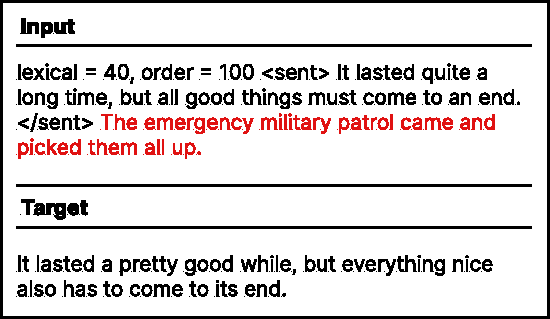
\includegraphics[width=.9\linewidth]{images/methods/kpar3-context-sample.pdf}
                \caption{\emph{(a)} Context Sample}
                \label{fig:kpar3-context}
            \end{subfigure}%
            \begin{subfigure}{.5\textwidth}
                \centering
                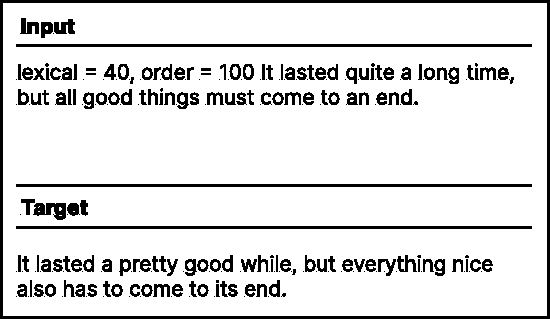
\includegraphics[width=0.9\linewidth]{images/methods/kpar3-non-context-sample.pdf}
                \caption{\emph{(b)} Non-context Sample}
                \label{fig:kpar3-non-context}
            \end{subfigure}
            \caption{Figure displays comparison between a paraphrase pair with context (a), and a paraphrase without context (b). The context portion in (a) is highlighted red for clarity. Furthermore, in (a), the <sent> tags denotes the text to be paraphrased. The target section refers to the desired output of text. Our dataset sample only contains examples like shown in (b). The terms `lexical' and `order' refer to the parameters used for determining paraphrase strength.}
            \label{fig:kpar3-sample-comparison}
        \end{figure}
        
        The original paper trains the model on the entire kPar3 dataset, taking between 384-768 GPU hours. Incapable of replicating the same compute periods, the finetuned model that I present is trained on our sampling of 100,000 documents, taking 14 GPU hours. Further specifications into the training arguments are provided in Appendix~\ref{append:training-args}. 

        Finally, to attack our documents, we apply paraphrasing attacks on the entire document with the parameters L40 and O40, describing a moderate paraphrase. Similarly, our generation strategy is top-$p$ sampling, where $p$ is 0.75, as suggested in the original paper \citep{krishna2023paraphrasing}. The paraphrasing is repeatedly recursively to assist in our understanding of the effects of recursive paraphrasing on the Maryland Watermark, our first research question.

        
    \subsection{Sentence-Based Paraphrasing}
        Opposing the prior method, we aim to separate the paragraph into sentences here and paraphrase each sentence independently. In this section, I will cover the algorithm and model that helps us answer \hyperref[sec:research-questions]{\textbf{RQ2}}.

        With regards to the model, we chose a model known as the \codefont{ChatGPT Paraphraser} \citep{chatgpt_paraphraser}. Similar to the paragraph model previously described, this is a model built off of T5, \codefont{T5-base} to be exact. The paraphraser is trained on a synthetic dataset of paraphrases produced by ChatGPT, hence the name. For brevity, I will refer to this model as \emph{$s$-paraphraser}.

        This model was chosen due to a lack of sentence-based models within research literature and consequent popularity of the model within the HuggingFace platform.

        As our attacking method, we complete sentence-based tokenisation with the help of the Natural Language Toolkit (NLTK) \citep{bird2009natural}. Each sentence is separated and passed to our paraphraser, similarly using top-$p$ sampling. The paraphrased sentences are connected together once more, as sentences, maintaining their order.

        The existence of $s$-paraphraser is precisely what we need, alongside our paragraph-based paraphraser, in order to evaluate differences between sentence-based and paragraph-based paraphrasers, our second research question.
    
    \subsection{Word Replacement}
        In order to answer our penultimate research question, we attempt attacking with the use of a word-replacement algorithm. Within this section, I will be discussing the implementation of the algorithm as well as the particular variations that we choose to evaluate.

        The algorithm is dependent on appropriately identifying the grammatical nature of each word, as to find an apt replacement. An immediate solution to this is available in the form of Flair's POS Tagger \citep{akbik2018coling}, which is a low-cost model that provides grammatical insight into a sentence.

        The POS tagger is paired with the WordNet \citep{wordnet1998fellbaum} library which recognises 155,327 distinct words. Linked to these recognised words, there is 117,597 sets of synonyms, known as Synsets. Note that two words can be linked to the same Synset. 

        With the knowledge of a word and its grammatical structure, we can apply word-replacement by searching the related Synset and selecting an option from here. Our selection from the Synset is a random sample, as the set is unordered. This synonym choice could be improved by picking the most similar word, according to word embedding model, such as Word2Vec.

        Hence, we can summarise our algorithm as follows:
        \begin{enumerate}
            \item \textbf{Tagging}: Grammatically tag the document with Flair's POS.
            \item \textbf{Select Words}: Select words to replace based on percentage or word-type.
            \item \textbf{Find Synonyms}: With respect to the selected words and grammar, collect potential synonyms.
            \item \textbf{Choose Synonym}: Randomly sample a choice from the synonym set.
            \item \textbf{Rebuild Document}: Rebuild the document, replacing the chosen words.
        \end{enumerate}

        The step outlined as Step (2) is where we introduce algorithm variations. With a tagged document, we could randomly replace a given percentage of the document. This has flaws as WordNet is not built for dealing with verb replacement of differing tenses. To deal with this, we could choose to replace all the nouns or adjectives. However, importantly, by limiting to certain grammar, we reduce the number of replaceable words.

        In this paper, we choose to attack with a \emph{noun-replacement} approach as well as \emph{25\% of words replacement} approach. Noun-replacement was chosen as it is the most common class of word recognised by WordNet, as mentioned in WordNet stats found in Appendix~\ref{append:wnet-stats}. The percentage attack is selected to match the green list fraction, as mentioned in Section~\ref{sec:watermark-implementation}. 

        The attack of this algorithm will provide exactly the results necessary to discuss the sufficiency of word-replacement algorithms with regards to Maryland Watermark removal effectively.

\section{Evaluation Stage}
    In order to answer any of our research questions, we need a way to numerically evaluate a watermark's strength and associating factors. Therefore, we come to the most important stage of our method. This section will discuss our evaluation strategy as well as the necessary metrics for understanding our results. The approach we have taken to evaluation is graphically outlined in Figure~\ref{fig:method-flow-chart}. 
    
    Our main topics are detection, similarity and perplexity. These topics are intended to measure watermark strength, paraphrase quality and text quality respectively. 
    
    \subsection{Watermark Detection}
        The metrics and formulas provided here are vital to understand the results presented in Chapter~\ref{chap:results}. This section begins with describing the Maryland method of detection followed by the equations and metrics for detection evaluation. These equations are precisely the way in which we measure the robustness of a watermark, pre- and post-attacks. The section will end with how to understand the metrics and gleam meaning from them.

        We begin with defining the $z$-score proposed by \citet{kirchenbauer2023watermark}, a statistical measure of standard deviation.
        \begin{definition}[Z-Score]
            Let $\gamma \in (0, 1)$. Let $T$ and $|s|_G$ denote the size of the vocabulary and number of green tokens in the document $s$.
            \begin{align*}
                z = \frac{|s|_G - T\gamma}{\sqrt{T\gamma(1 - \gamma)}},
            \end{align*}
            where $\gamma$ represents the fraction of the vocabulary which are green tokens.
        \end{definition}
        $Z$-Scores can be used to determine how irregular a result is. For our case, this formula is used to determine if a document is watermarked. Specifically, we call a document \textbf{watermarked} if the $z$-score is 4 or greater. The primary takeaway is that this result is strongly dependent on the green fraction as well as the \emph{detectable} green tokens. 

        Whilst a document may be watermarked, it is up to the Maryland detection algorithm to find the green tokens which prove the watermarking. The code and implementation for the detection algorithm was provided by \citet{kirchenbauer2023watermark}. The algorithm determines the colour of a token through splitting the vocabulary in the same way as the watermarking process, through the hash of the previous token. Figure~\ref{fig:maryland-detection-process} provides a visual explanation of the process for a single token.

        \begin{figure}[ht]
            \centering
            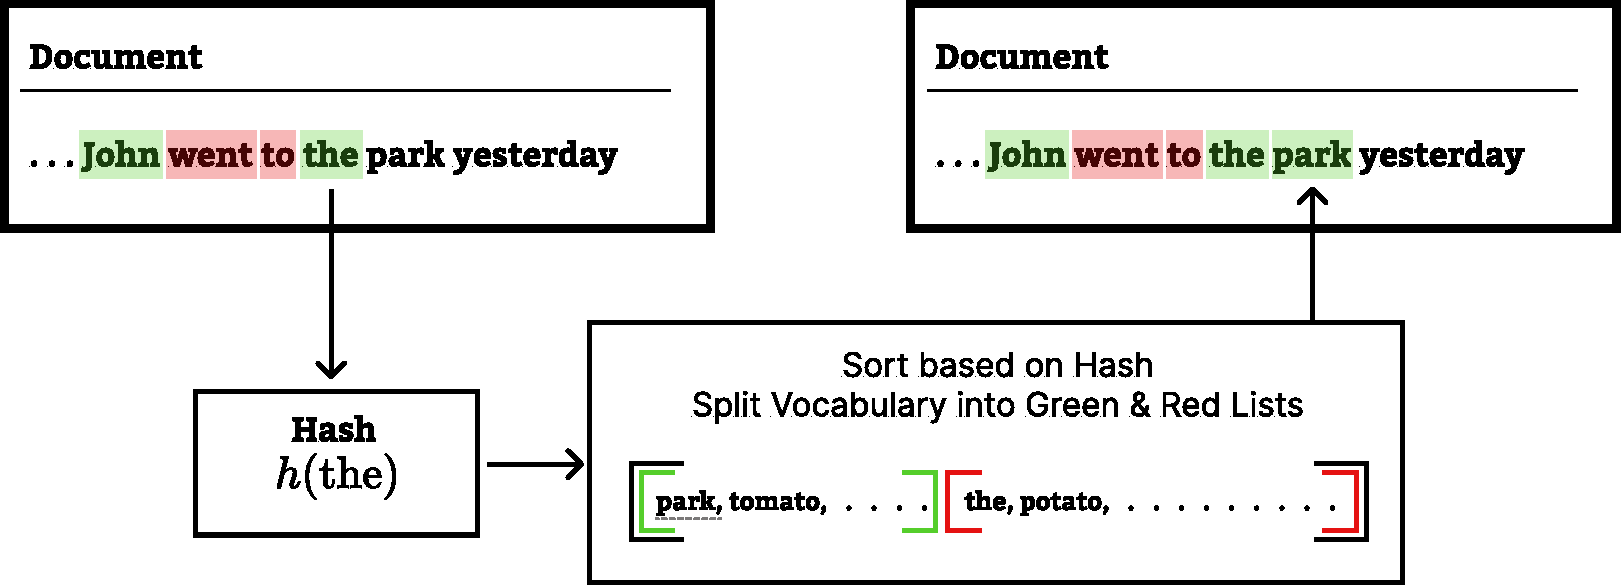
\includegraphics[width=1\linewidth, keepaspectratio]{images/methods/maryland-detection-process.pdf}
            \caption{Figure shows the process of determining token colour of the token \textbf{park}. We hash the previous token \textbf{the} in order to sort our vocabulary. Furthermore, the green and red list is dynamically created based on the hash key, so it is harder to crack for bad actors. Importantly, tokens which are green, such as \textbf{the}, only need to be in the green list based on the hash of the token before it.}
            \label{fig:maryland-detection-process}
        \end{figure}

        Once the entire document is classified into red and green tokens, the green tokens are counted and used for the $z$-score evaluation.

        As mentioned in Section~\ref{sec:tokenisation}, the detection algorithm must know the tokeniser for generation. In particular, they must know the vocabulary in order to split the tokens correctly and identify which colour that a token belongs to. The uniqueness of tokenisation means that if the generation model and respective tokenisation function are unknown, the detection algorithm will not be capable of correctly identifying the watermark. This is a problem that leads to the watermark failing the \emph{agnostic} property of watermarking.

        The detectable green tokens are precisely the area in which the attacks take place. These attacks result in two primary types of errors, Type-$I$ and Type-$II$ errors. 
        
        A Type-$I$ refers to falsely detecting a human-generated document as a machine-generated document, also known as a \emph{False Positive}. Similarly, a Type-$II$ refers to detecting a machine-generated document as human-generated, also known as \emph{False Negative}. Given that one of the major goals is to minimise the number of Type-$I$ errors, as mentioned in Chapter~\ref{chap:results}. The metric used to evaluate the number of false positives is known as the \emph{False Positive Rate}.

        \begin{definition}[False Positive Rate]
            Let $N$ and $FP$ be the number of non-watermarked and number of false positives respectively. We define the \emph{False Positive Rate} (FPR) as follows:
            \begin{align*}
                \text{FPR} = \frac{FP}{N}
            \end{align*}
        \end{definition}

        While FPR ensures that we do not incorrectly mark human documents, we also wish to make sure that we can correctly identify watermarked documents as watermarked. For this, the notion of a \emph{True Positive} is introduced, which is a watermarked document correctly classified as watermarked. Hence, we introduce a neighbouring metric, known as the \emph{True Positive Rate}. 

        \begin{definition}[True Positive Rate]
            Let $P$ and $TP$ be the number of watermarked documents and the number of true positives respectively. Then we define the \emph{True Positive Rate} (TPR) as follows:
            \begin{align*}
                \text{TPR} = \frac{TP}{P},
            \end{align*}
            This metric is also known as \emph{recall}.
        \end{definition}

        % Really want some sort of separation here. Moving from stats to particular metrics now.
        On their own, these metrics are useful. However, we can create even more visualisations from these introduced metrics that help us understand our watermark. A popular visualisation is the \emph{Area under the Receiver Operating Characteristic} (AUROC), which measures the TPR against the FPR. By repeatedly altering our z-score threshold of 4.0, we can re-evaluate the detection ratings and help determine the strength of our watermark. In the end, within this visualisation, we wish to see the curve maximising the area under the curve.
        
    \subsection{Document Similarity}
        \label{sec:document-similarity}
        While we can evaluate the removal of a watermark, it is useful to have a notion of cost in the removal. This section will discuss how to understand the cost of an attack and our implementation of similarity metric.

        By placing confidence in our generation LLM (Mistral Model) alongside the imperceptibility of the Maryland Watermark, we can consider cost by measuring similarity to the original document. Under the assumption that the original document is the ideal response to the prompt, we consider the similarity to the original document to represent the cost of attacking.

        The chosen measure is cosine similarity, as that is convention in NLP. Notably, cosine similarity requires vector representations of our documents. Our major choice design choice arrives in determining the vector representations of our documents. 

        Technically, cosine similarity is not the similarity between documents but rather the similarity between the document embeddings with respect to a given model. This difference is significant as models produce unique representations, leading to different similarities. Furthermore, similarity does not respect paraphrases particularly well, as can be seen in Example~\ref{example:paraphrase-vs-paragraph}.

        \begin{example}
            \label{example:paraphrase-vs-paragraph}
            The sentences below are similar sentences, wherein (2) and (3) are human paraphrases.
            \begin{enumerate}[label=(\arabic*)]
                \item I take my cat on a walk on Wednesdays in Central Park.
                \item I take my dog on a walk on Wednesdays in Central Park.
                \item Every Wednesday, I walk my dog in the centre of New York City.
            \end{enumerate}
            Using the HuggingFace model \codefont{all-mpnet-base-v2}, the highest-rated document embedding model, we see that sentences (1) and (2) are more similar, despite (2) and (3) being a paraphrase pair, with respect to the cosine measure.
        \end{example}

        In an attempt to feel confident with our document embeddings and consequent cosine similarities, we will be using an embedding model trained on paraphrastic pairs. \citet{wieting2023paraphrastic} provides exactly this model as well as stating results proving its effectiveness. \citet{krishna2023paraphrasing} uses this model for similarity and, from analysis on human-paraphrases, states that a similarity of 0.76 is a sufficient score to maintain the original meaning.

        For each attack, we evaluate every attacked document against the original, unaltered, document. This evaluation is focused on understanding how much the original meaning of a document is degraded through attacking, helping us understand the cost of attacking our models.

    \subsection{Perplexity Measure}
        As we place confidence in the similarity measure, we can also apply an adjacent metric. This section discuss another evaluation metric used to determine the quality of a text, helping us further understand the cost of attacking.

        Within Natural Language Processing, we use a measure known as perplexity that allows us to gauge how likely a model is to produce a document.

        \begin{definition}[Perplexity]
            Let $s$ be a document of length $n$ and let $s_i$ denote the $i$th token. We define the \emph{perplexity} function PPL as follows:
            \begin{align*}
                \text{PPL}(s) = \exp\Bigg(-\frac{1}{n}\sum_i^n\log p(s_i | s_{<i})\Bigg),
            \end{align*}
            where $p$ is the probability of a token given the previous tokens from a given model. Numerically, the model is `unsurprised' by a generated document when the perplexity is closer to 1.
        \end{definition}

        The probability function $p$ is entirely dependent on the current language model, hence each model will give a different perplexity for a document. To define a relative metric, some papers \citep{kirchenbauer2023watermark, giboulot2024watermax, he2024watermarks} have intelligently used the same language model to calculate perplexity, \codefont{OPT-2.7B}. To allow our paper to have comparable results, we also match this convention and use this language model for perplexity. 
        
        If we operate under the assumption that the language model used for perplexity is a strong language model, we know that a low-valued perplexity represents a high quality document.

        The perplexity is computed on all documents, both attacked and unaltered. 


%==================================================================================================================================
\chapter{Results} 
\label{chap:results}
In this section, we try to answer our primary research questions provided the results we generated through the implementation outlined in Chapter~\ref{chap:method}. To aid the reader, these are the research questions that we are looking to answer: 
\begin{enumerate}[label={\textbf{RQ\arabic*}:}, leftmargin=4em]
    \item Does paraphrasing recursively degrade accuracy in detection of the Maryland Watermark?
   \item Is sentence-based paraphrasing more effective than paragraph-based paraphrasing when dealing with removal of the Maryland Watermark?
    \item Is a low-cost, word-replacement algorithm sufficient to remove the Maryland Watermark? 
    \item Are the attacking methods feasible for use within an academic context with respect to the Maryland Watermark?
\end{enumerate}

\section{Recursive Paraphrasing}
    In order to answer our first research question, we investigate the power of recursive paraphrasing. In this section, we aim to see the strength of the watermark varying after each iteration. Furthermore, we wish to understand the cost of repeatedly paraphrasing. These results will help us see whether recursive paraphrasing is an effective tool with regards to removing the Maryland Watermark. 

    \begin{figure}[ht]
        \centering
        \captionsetup[subfigure]{labelformat=empty}
        \begin{subfigure}{.495\textwidth}
            \centering
            \includegraphics[width=\linewidth]{images/results/roc/roc-curve-para.pdf}
            \caption{\emph{(a)} Paragraph-Based Paraphrasing}
            \label{fig:para-roc}
        \end{subfigure}
        \begin{subfigure}{.495\textwidth}
            \centering
            \includegraphics[width=\linewidth]{images/results/roc/roc-curve-sent.pdf}
            \caption{\emph{(b)} Sentence-Based Paraphrasing}
            \label{fig:sent-roc}
        \end{subfigure}
        \caption{Figure portrays the ROC curves of the documents after (a) Paragraph-Based Paraphrasing and (b) Sentence-Based Paraphrasing. The legend contains information about AUROC as well the respective iteration of each curve. Finally, the dashed line is a random classifier that highlights a lower-bound on performance. The evaluation is completed on 996 documents, half of which are watermarked with $\delta = 5, \gamma = 0.25$.}
        \label{fig:roc-para-sent-comparison}
    \end{figure}

    Using the AUROC graphs, as seen in Figure~\ref{fig:roc-para-sent-comparison}, we see that repeatedly paraphrasing does alter the detection performance. The graphs, composed of $z$-scores and altering thresholds, highlight worse performance as the curves tend towards the linear curve. Interestingly, both paraphrasing methods display the same detection trend, in which the first paraphrase is the most effective in removing the watermark. Meanwhile, the second iteration, contrary to intuition, actually has a stronger watermark compared to the first paraphrase.

    The irregularity of the second iteration is representative of the unpredictability in Maryland Watermark, where the green and red tokens are split entirely based on the hashing function of tokens. Specifically, this result shows that we cannot guarantee continual degradation in watermark detection as we recursively paraphrase. 

    Beyond detection performance, we also look to understand the textual cost of the repeated paraphrasing. Within Table~\ref{table:recursive-paraphrase-table}, there is a degradation in similarity as we continue to paraphrase, with both paragraph-based and sentence-based attacks. Given that the similarity is measured against the base, unaltered document, the decreasing scores suggest that we are losing our original meaning.

    \begin{table}[ht]
        \centering
        \begin{tabular}{c|cc}
        \multirow{2}{*}{Documents}  & \multicolumn{2}{c}{Similarity ($\uparrow$)} \\ \cline{2-3} 
        & \multicolumn{1}{c|}{$p$} & $s$ \\ \hline
        First Paraphrase & 0.820 & \textbf{0.856} \\
        Second Paraphrase & 0.731 & \textbf{0.820} \\
        Third Paraphrase & 0.671 & \textbf{0.785} 
        \end{tabular}
        \caption{Table represents evaluation completed on 996 documents for each iteration, of which half are watermarked as per the arguments in the methods chapter. The segments $p$ and $s$ denote the paragraph-paraphraser and sentence-paraphraser respectively. The direction of the similarity arrow shows that we want a higher score from this evaluation. The numbers in bold denote the best score within their evaluation segment, for each iteration.}
        \label{table:recursive-paraphrase-table}
    \end{table}

    Furthermore, according to \citet{krishna2023paraphrasing}, a document similarity of less than 0.76 means that the original similarity has been lost. In terms of binary classification, the paragraph-based paraphraser fails to maintain clarity in the latter two paraphrases.

    Ultimately, to answer our first research question, paraphrasing recursively does not predictably degrade accuracy in the detection of the Maryland Watermark. Furthermore, we see that repeated paraphrasing can distance a document from its original meaning, potentially lowering the value of a document.
    
\section{Sentence-Paraphrasing against Paragraph-Paraphrasing}
    \label{sec:sentence-against-paragraph}
    For our second research question, we look towards a comparison between sentence-based and paragraph-based paraphrasing with regards to an effective removal of the Maryland Watermark. To answer our question, we view the watermarking confidence paired with our described cost metrics. 

    Viewing Table~\ref{table:sentence-against-paragraph-comparison}, we see that the paragraph-based paraphraser is \emph{marginally} better at removing the watermark with respect to Type-$I$ and Type-$II$ errors. In fact, with the \citet{kirchenbauer2023watermark} threshold of 4.0, there is no Type-$II$ errors. There is a small difference with regards to TPR, Type-$I$ errors, which I believe is a reflection of paragraph-restructuring potential that $p$-paraphraser contains.

    \begin{table}[ht]
        \centering
        \begin{tabular}{c|c|c|c|c}
            Paraphrase Attacking Method & TPR (\%) & TNR (\%) & Perplexity ($\downarrow$) & Similarity ($\uparrow$) \\ \hline
            Paragraph-Based & \textbf{1.606} & \textbf{100} & \textbf{19.530} & 0.820 \\
            Sentence-Based & 3.815 & \textbf{100} & 24.889 & \textbf{0.856}
        \end{tabular}
        \caption{Table displays results evaluated on 996 documents for each iteration. Half of the documents are watermarked as per the arguments in the methods chapter. TPR and TNR are calculated with respect to the $z$-score threshold of 4.0, acting as a classification boundary. The arrows point in the direction of ideal results. The best result for each metric is in bold.}
        \label{table:sentence-against-paragraph-comparison}
    \end{table}

    One of the key results within Table~\ref{table:sentence-against-paragraph-comparison} is perplexity. It is clear that the $p$-paraphraser can provide higher quality text, as per the \codefont{OPT-2.7B} model. However, despite the greater text quality, the sentence paraphraser retains higher similarity to the original document.

    To answer our question, as to whether sentence-based or paragraph-based is more effective at watermark removal, I would argue that the choice of paraphraser does not matter. Although $p$-paraphraser performs slightly better, I believe this to be a difference in model quality as the $p$-paraphraser is finetuned on a superior model to $s$-paraphraser.

\section{Word Replacement Sufficiency}
    To answer our penultimate question, we look towards our two variations of word-replacement attacks. To analyse the sufficiency of our algorithm, we consider the TPR and TNR metrics at the Kirchenbauer $z$-score threshold of 4.0.

    From Table~\ref{table:word-replacement-comparison}, we quickly see that noun-replacement is insufficient to break the Maryland Watermark. The high TPR shows that we correctly identify almost all watermarked documents and do not misidentify any non-watermarked documents. In fact, even the 25\% Word Replacement is not sufficient, which is interesting precisely because 25\% is how much of the vocabulary is to be in the green list for each token ($\gamma = 0.25$). 

    \begin{table}[ht]
        \centering
        \begin{tabular}{c|c|c|c}
            Replacement Method & TPR (\%) & TNR (\%) & Perplexity ($\downarrow$) \\ \hline
            Noun-Replacement & 95.783 & 100 & 69.571 \\
            Percentage-Replacement (25\%) & 39.759 & 100 & 105.164
        \end{tabular}
        \caption{Table displays metrics evaluated of 996 documents, for each replacement method. The TPR and TNR values are complete according to the $z$-score of 4.0 Furthermore, the arrow denotes that you want perplexity as a lower value, as close to 1 as possible. The percentage-replacement method is completed with replacing 25\% of words in each document.}
        \label{table:word-replacement-comparison}
    \end{table}

    Interestingly, the change in words does have a noticeable impact on the $z$-scores, as can be seen in Figure~\ref{fig:noun-replacement-z-score}, showing the effect with an noun-replacement attack. Figure~\ref{fig:percentage-replacement-z-score} shows the same graph but using the percentage-replacement attack. The vertical distance from the ideal linear line reflects the impact of attacking with word replacement. It seems as though, for both methods, that the z-score is typically reduced but it is simply not sufficient. 
    
    A positive result, for the Maryland Watermark, is the lack of difference in $z$-scores within the non-watermarked documents, as seen by the orange points in figures \ref{fig:noun-replacement-z-score}, \ref{fig:percentage-replacement-z-score}. This result reflects that the replacement methods cannot lead to \emph{spoofing} attacks, as mentioned in Section~\ref{sec:other-watermarks}, and undermine the credibility of the Maryland Watermark.
    
    \begin{figure}[ht]
            \centering
            \captionsetup[subfigure]{labelformat=empty}
            \begin{subfigure}{\textwidth}
                \centering
                \includegraphics[height=5cm, width=\linewidth, keepaspectratio]{images/results/z-score/noun word-replacement.pdf}
                \caption{\emph{(a)} Noun-Replacement Attack}
                \label{fig:noun-replacement-z-score}
            \end{subfigure}
            \begin{subfigure}{\textwidth}
                \centering
                \includegraphics[height=5cm, width=\linewidth, keepaspectratio]{images/results/z-score/percentage word-replacement.pdf}
                \caption{\emph{(b)} Percentage (25\%) Replacement Attack}
                \label{fig:percentage-replacement-z-score}
            \end{subfigure}
            \caption{Figure displays the $z$-Score of 996 documents after the effects of attacking with (a) noun-replacement and (b) percentage-replacement. The documents are orange and blue to denote whether they are non-watermarked or watermarked. In terms of an (x,y) frame, the x-coordinate refers to the $z$-score before noun-replacement whereas the y-coordinate refers to the $z$-score refers after noun-replacement. The distance of a datapoint from the dashed line represents the impact of attacking. Finally, the red-lines represent the $z$-score threshold of 4.0.}
            \label{fig:kpar3-sample-comparison}
    \end{figure}

    Even with the lacking capacity to remove the watermark, the cost of completing word-replacement is not negligible. As compared to results in Table~\ref{table:sentence-against-paragraph-comparison}, the word-replacement documents have approximately 3$\times$ the perplexity, reflecting the poor textual quality of the documents. As a benchmark, the mean perplexity of the human-written documents is 18.632 (to 3 s.f.).

    Fortunately, we can now provide a clear answer to the question as to whether a low-cost, word-replacement algorithm is appropriate for removing the Maryland Watermark. The noun-replacement variation is certainly not capable of removing the watermark whereas the percentage-replacement has the potential for removal but comes at a significant textual quality cost. Hence, low-cost word-replacement algorithms are not sufficient in removing the Maryland Watermark.

\section{Feasibility of Attacking Techniques}
    We consider our final question as a culmination of the previous questions. This question deals with the feasibility of using these attacking techniques in a realistic pipeline to evade watermark detection.

    Immediately, we have established that word-replacement does not effectively avoid detection, nor does it provide high quality text as an output. Hence, we do not consider it as a feasible approach. 

    On the other hand, the paragraph-based paraphrasing produces high quality and effectively evades detection, being correctly detected only around 2\% of the time. However, this is a heavy-duty paraphrasing model which requires running a 1.5B parameter causal model. As mentioned in \citet{kirchenbauer2023watermark}, with access to a high quality paraphraser without a watermark, it is probably easier to generate the text outwith the watermarking model and avoid having to paraphrase.

    Unlike the other attacking methods, using the $s$-paraphraser remains a feasible technique. 

    The sentence-based paraphraser performed similarly to the paragraph-paraphraser at a fraction of the memory costs, as a model of 223M parameters. By approximation and typical memory costs, this is around 1GB of RAM to run inference at most. Hence, when detection is only achieved approximately 4\% of the time, sentence-based paraphrasing becomes a realistic technique for evading detection in an academic context, particularly given that the perplexity is not largely worse than the mean perplexity of human-written essays, at 18.632.

%==================================================================================================================================
\chapter{Conclusion}
% Things to discuss:
% \begin{enumerate}
%     \item What we created to investigate.
%     \item The questions that we aimed to answer.
%     \item The answers to our questions.
%     \item Limitations in the project - both computational and also metrics.
%     \item Future directions / what I would like to investigate with more time. 
% \end{enumerate}

In this paper, we attempted to remove the \emph{Maryland Watermark} from AI-generated documents with two types of paraphrasers as well as a word-replacement algorithm. We used a high-quality LLM to generate 1000 documents and completed an analysis focused on answering research questions surrounding paraphrasing, word-replacement and the academic use of watermarks.

The two paraphrasers, sentence-based and paragraph-based, helped us answer our first research question discussing the impact of recursive paraphrasing on detection accuracy of the Maryland Watermark. Our results showed that the detection accuracy does not linearly degrade with paraphrase iterations and that detection accuracy can, in fact, increase between iterations. To put this result into one sentence: you \emph{cannot} confidently repeatedly paraphrase under the assumption that detection accuracy will decrease.

Our two paraphrasers were compared in our second question which dealt with the quality of watermark removal. Assisted by textual quality metrics, we determined that the style of paraphraser was \emph{insignificant in practice} with regards to removing the watermark. However, we did note that it would be worth re-evaluating again with more comparable paraphrasers with regards to the base model.

Our most conclusive result was for our third question, focused on whether replacing words was a sufficient technique to remove the Maryland Watermark. Through our noun-replacement and percentage-replacement algorithms, we discovered results that clearly show that word-replacement is \emph{insufficient} and the Maryland Watermark is robust against such-techniques. Under noun-replacement, we saw that detection accuracy, with recommended detection conditions, dropped from 100\% to 96\%. 

We summarise our results within our final question, discussing the feasibility of our attacking techniques in an academic context. Even while acknowledging the computational costs for students, we determine that the sentence-based paraphraser is a usable technique to evade detection when the Maryland Watermark is used. The paraphraser retains the textual quality as well as the original meaning, according to our cost-focused metrics.

\section{Limitations}
    Despite being fortunate to own a graphics card with significant VRAM, it was not quite enough to run some of the greater models. One notable issue was the inability to use the DIPPER Model, the superior paragraph-based paraphraser outlined in Section~\ref{sec:paragraph-paraphraser}. This meant training another model, of lower quality.

    In a similar vein, I did not have the compute time to finetune models or generate massive amounts of evaluation data. This meant the analysis was completed on a smaller amount of data than I would have liked. However, I was fortunate to have the opportunities that I did have and managed to produce results nonetheless.

    In all honesty, the limitation that I felt the greatest was with regards to paraphrase similarity. As mentioned in Section~\ref{sec:document-similarity}, the similarity measure deals with document similarity, not so much paraphrase similarity. Countermeasures were put in place, like picking a model specifically for paraphrase similarity, but it did not feel sufficient. As it stands, there is few appropriate numerical paraphrase metrics as even the common ones, like BLEU, are not seen as conclusive evidence. This limitation led to a lack of confidence in understanding if a paraphrased-document has kept its original meaning, something important within our analysis. 

\section{Future Work}
    Amongst all the limitations, I still feel that I proud of the work that I produced and would have been happy to continue working on this topic. With regards to my existing research questions, I would have liked the opportunity to finetune my own sentence-based paraphraser, as it would have allowed a more comparable analysis between our paraphrasing styles.

    Similarly, I would have liked more time to finetune the paragraph-based paraphraser, to achieve a quality closer to the original model, DIPPER.
    
    Outwith my existing research questions, there are two avenues into which I would like to expand my analysis, which I propose below as further research questions
    \begin{enumerate}[label={\textbf{RQ\arabic*}:}, leftmargin=4em]
        \setcounter{enumi}{4}
        \item Does the use of a sliding-window for $z$-score calculations provide greater accuracy for detection of documents that contain AI-generated text? 
        \item Do the previously mentioned paraphrasing attacks succeed against a semantic-influenced watermarking technique?
    \end{enumerate}

    The first of these research questions deals with the issue of embedding AI-generated text within largely human-written documents. Meanwhile, the second question is simply an analysis of an existing technique which is especially designed to be robust against paraphrasing. The second question is interesting because, without paraphrasing, more intelligent attacking methods may be required.


%==================================================================================================================================
%  APPENDICES  

\begin{appendices}

\chapter{Appendices}
\section{Paraphraser-Based Paraphaser | Training Arguments}
    \label{append:training-args}
    The following arguments refer to the entire training arguments used for training our paraphraser.
    
    \begin{lstlisting}[language=json,firstnumber=1]
    {
        "learning_rate": 1e-4,
        "bf16": True,
        "num_train_epochs": 2,
        "auto_find_batch_size": True,
        "generation_num_beams": 2,
        "generation_max_length": 200
    }
    \end{lstlisting}
    More information is publicly available on the HuggingFace links: \href{https://huggingface.co/SamSJackson/paraphrase-dipper-no-ctx}{paraphrase-no-ctx}, \href{https://huggingface.co/datasets/SamSJackson/kpar3-no-ctx}{kpar3-no-ctx} 

\section{WordNet Stats}
    \label{append:wnet-stats}
    The following information is present on the WordNet website: \href{https://wordnet.princeton.edu/documentation/21-wnstats7wn}{Stanford WordNet Stats}.
    \begin{table}[ht]
        \centering
        \begin{tabular}{@{}p{0.25\linewidth}p{0.2\linewidth}p{0.2\linewidth}p{0.2\linewidth}@{}}
            \toprule
            \textbf{POS} & \textbf{Unique} & \textbf{Synsets} & \textbf{Total} \\ \midrule
             & \textbf{Strings} &  & \textbf{Word-Sense Pairs} \\ \midrule
            \multicolumn{1}{l|}{Noun} & 117097 & 81426 & 145104 \\
            \multicolumn{1}{l|}{Verb} & 11488 & 13650 & 24890 \\
            \multicolumn{1}{l|}{Adjective} & 22141 & 18877 & 31302 \\
            \multicolumn{1}{l|}{Adverb} & 4601 & 3644 & 5720 \\
            \multicolumn{1}{l|}{Totals} & 155327 & 117597 & 207016 \\ \bottomrule
        \end{tabular}
    \end{table}

\end{appendices}

%==================================================================================================================================
%   BIBLIOGRAPHY   

% The bibliography style is abbrvnat
% The bibliography always appears last, after the appendices.

\bibliographystyle{abbrvnat}

\bibliography{l4proj}

\end{document}
